\documentclass[5pt]{article}
\usepackage{multicol,multirow}
\usepackage{graphicx} % Required for inserting images
\usepackage[margin=0.45cm]{geometry}
\usepackage{xcolor}
\usepackage{array}

\definecolor{LightGray}{gray}{0.9}

\newcolumntype{L}{>{\footnotesize}l}
\newcolumntype{C}{>{\ttfamily\footnotesize}l}

\usepackage{amsmath,esint}
\usepackage{mathtools}
\usepackage{relsize}
\usepackage{mathtools}
\usepackage{nccmath}
\usepackage[inline]{enumitem}
\usepackage{algpseudocode}

\usepackage{empheq}
\usepackage{amsfonts}

\usepackage{tkz-euclide}
\usepackage{tikz}

\usepackage{minted}

\newenvironment{amatrix}[1]{%
  \left[\begin{array}{@{}*{#1}{c}|c@{}}
}{%
  \end{array}\right]
}

\DeclarePairedDelimiter\abs{\lvert}{\rvert}%
\DeclarePairedDelimiter\norm{\lVert}{\rVert}%
\newcommand{\universalSet}{\mathbb{U}}

\makeatletter
\let\oldabs\abs
\def\abs{\@ifstar{\oldabs}{\oldabs*}}

\newcommand{\tr}[3]{
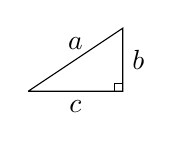
\begin{tikzpicture}[scale=0.40]
    \coordinate [] (A) at (-1.5cm,-1.cm);
    \coordinate [] (C) at (1.5cm,-1.0cm);
    \coordinate [] (B) at (1.5cm,1.0cm);
    \draw (A) -- node[above] {$a$} (B) -- node[right] {$b$} (C) -- node[below] {$c$} (A);
    \draw (1.25cm,-1.0cm) rectangle (1.5cm,-0.75cm);
\end{tikzpicture}
}

\begin{document}

\newtheorem{theorem}{Theorem}
\newtheorem{lemma}{Lemma}
\newtheorem{properties}{Properties}
\newtheorem{axiom}{Axiom}


\begin{center}
     \Large{\textbf{Discrete Mathematics}}\\
     \small{Last Update: \today}\hfill\small{\textcopyright Maximilien Notz \the\year{}}
     \noindent\rule{20.2cm}{0.4pt}
\end{center}

\begin{multicols}{2}
\setcounter{secnumdepth}{0}
\subsection{General Terminology}
\begin{tabular}{L L}
    Descriptive statistics & Summarizing, organizing and describing data.\\
    Inferential statistics & using probability theory to extrapolate conclusions\\
                           & from data.\\
    Population & A collection of all individuals or items of interest.\\
    Sample & A subset of the population.\\
    statistic & A numerical property of a sample.\\
    Parameter & A numerical property of the whole population.\\
    Variable & A characteristic or measurement of interest for the\\
             & individuals in a population.\\
    Data & The values of the variables.\\
    Quantitative variable & A variable that can be measured numerically.\\
    Qualitative variable & A variable that can be categorized based on some\\
                         & characteristic or attribute.\\
    Discrete variable & A quantitative variable that can take on only a finite\\
                      & or countable number of values.\\
    Continuous variable & A quantitative variable that can take on any value in\\
                         & an interval of real numbers.\\
    Nominal variable & A qualitative variable that has no natural ordering.\\
    Ordinal variable & A qualitative variable that has a natural ordering.\\
    Frequency & The number of times a value or category occurs.\\
    Relative frequency & Normalized frequency, expressed as a percentage.\\
    frequency table & A table that displays the frequency or relative\\
                     & frequency of each value.\\
    Rounding & Carry the final answer with one more decimal place\\
             & than the data with the least number of decimal places.\\
\end{tabular}

\subsection{Sampling Methods}
There are 2 main types of sampling methods: random and non-random.\\
\begin{tabular}{LL}
  Simple random & Every individual in the population has an equal chance o\\
                & being selected.\\
  Stratified & The population is divided into subgroups (strata) based on\\
            & some characteristic, and a random sample is taken from\\
            & each stratum.\\
  Cluster & The population is divided into clusters, and a random\\
          & sample of clusters is selected. All individuals in the selected\\
          & clusters are included in the sample.\\
  Systematic & A random starting point is selected, and then every $k^{th}$\\
             & individual is selected from the population.\\
  Convenience & The sample is selected based on convenience or accessibility.\\
\end{tabular}

\subsection{Levels of Measurement}
\begin{tabular}{LL}
  Nominal  & Nornumerically meaningfull(labels).\\
  Ordinal  & Can order (star rating).\\
  Interval & Distance between values is meaningful.\\
  Ratio    & Has a definite zero, ratios are meaningful (e.g., height, time)\\
\end{tabular}

\subsection{Stat Formulas}
\begin{tabular}{LL}
  Interquartile range(IQR) & $IQR=Q_3-Q_1$\\
  Range                    & $R=x_{max}-x_{min}$\\
  Percentile Position      & $P_k=\frac{k(n+1)}{100}$\\
  Sample Mean              & $\bar{x}\approx\frac{\sum_{i=1}^{n}x_i}{n}$\\
  Population Mean          & $\mu$\\
  Median                   & The middle value of a sorted data set.\\
  Mode                     & The most frequently occurring value in a data set.\\
  Range                    & $R=x_{max}-x_{min}$\\
  Sample Variance          & $\sigma^2=\frac{\sum_{i=1}^{n}(x_i-\bar{x})^2}{n-1}$\\
  Population Variance      & $\sigma^2=\frac{\sum_{i=1}^{N}(x_i-\mu)^2}{N}$\\
  Standard deviation       & $\sigma=\sqrt{\sigma^2}$\\
  Z-score                  & $z=\frac{x-\bar{x}}{\sigma}$\\
  Skewness                 & $Sk=\frac{n}{(n-1)(n-2)}\sum_{i=1}^{n}\left(\frac{x_i-\bar{x}}{\sigma}\right)^3$\\
\end{tabular}

\subsection{Probabilities}
A probability quantifies the chance that an event occurs. A probability must respect the kolmogorov axioms listed below.\\
\begin{enumerate*}
  \item $\mathbb{P}(A) \geq 0, \forall A \in S$\\
  \item $\mathbb{P}(S) = 1$\\
  \item $\mathbb{P}(\bigcup_{i=1}^n A_i) = \sum_{i=1}^n \mathbb{P}(A_i)$ if $A_i \cap A_j = \emptyset$ for all $i \neq j$.\\
\end{enumerate*}
\vspace{1pt}
\begin{tabular}{LL}
  Experiment   & A process that leads to one of several possible outcomes.\\
  Outcome      & The result of a single trial of an experiment.\\
  Event        & A collection of one or more outcomes.\\
  Sample space & The set of all possible outcomes of an experiment. Notatied $S$.\\
\end{tabular}
\begin{tabular}{LL}
  Equally likely outcomes & $\mathbb{P}(A) = \frac{|A|}{|S|}$\\
  Expected value          & $\mathbb{E}(X)\equiv \sum_{i=1}^n x_i \mathbb{P}(x_i)=\mu$\\
  Conditional probability & $\mathbb{P}(A|B)=\frac{\mathbb{P}(A\cap B)}{\mathbb{P}(B)}$, $\mathbb{P}(A)$ given $B$ occured. \\
  Additive rule           & $\mathbb{P}(A\cup B)=\mathbb{P}(A)+\mathbb{P}(B)-\mathbb{P}(A\cap B)$\\
  Multiplicative rule     & $\mathbb{P}(A\cap B)=\mathbb{P}(A|B)\mathbb{P}(B)$\\
  Complement inverse      & $\mathbb{P}(A) + \mathbb{P}(A') = 1$
\end{tabular}

\subsubsection{Independent events}
knowing one occurred does not change the chance of the other.
\begin{itemize*}
  \item $\mathbb{P}(A|B) = \mathbb{P}(A)\;\;$
  \item $\mathbb{P}(A\cap B) = \mathbb{P}(A)\mathbb{P}(B)$
\end{itemize*}

\subsubsection{Mutually exclusive events}
events cannot occur together.\\
\begin{itemize*}
  \item $A\cap B = \emptyset\;\;$
  \item $\mathbb{P}(A\cap B) = \emptyset$
\end{itemize*}

\subsubsection{Sample space representations}
listing, tree diagram, Venn diagram.

\subsubsection{Contingency tables}

\end{multicols}
\subsection{General Tips}
\begin{itemize*}
    \item $\sum_{i=1}^{n}i=\frac{n(n+1)}{2}$
    \item $\sum_{i=1}^{n}i^2=\frac{n(n+1)(2n+1)}{6}$
    \item $\sum_{i=1}^n r^i=\frac{r(1-r^n)}{1-r}$ for $r \neq 1$
    \item $\sqrt{x^2}=|x|,x\in\mathbb{R}$
    \item $(\sqrt{x})^2=x, x\geq 0$
    \item $\cos{\theta}=\frac{e^{i\theta}+e^{-i\theta}}{2}$
    \item $\sin{\theta}=\frac{e^{i\theta}-e^{-i\theta}}{2i}$
    \item $e^{i\theta}=\cos{\theta}+i\sin{\theta}$
    \item $(a+b)^3=a^3+b^3+3ab(a+b)$
    \item $(a-b)^3=a^3-b^3-3ab(a-b)$
    \item $a^3+b^3=(a+b)(a^2-ab+b^2)$
    \item $a^3-b^3=(a-b)(a^2+ab+b^2)$
\end{itemize*}
\end{document}
